\documentclass[dvipdfmx,autodetect-engine,titlepage]{jsarticle}
\usepackage[dvipdfm]{graphicx}
\usepackage{ascmac}
\usepackage{fancybox}
\usepackage{listings}
\usepackage{plistings}
\usepackage{itembkbx}
\usepackage{amsmath}
\usepackage{amssymb}
\usepackage{amsfonts}
\usepackage{svg}
\usepackage{url}
\usepackage{graphics}
\usepackage{listings,jvlisting}

\lstset{
  basicstyle={\ttfamily},
  identifierstyle={\small},
  commentstyle={\smallitshape},
  keywordstyle={\small\bfseries},
  ndkeywordstyle={\small},
  stringstyle={\small\ttfamily},
  frame={tb},
  breaklines=true,
  columns=[l]{fullflexible},
  numbers=left,
  xrightmargin=0zw,
  xleftmargin=3zw,
  numberstyle={\scriptsize},
  stepnumber=1,
  numbersep=1zw,
  lineskip=-0.5ex
}

\textheight=23cm
\renewcommand{\figurename}{図}
\renewcommand{\tablename}{表}
\newenvironment{code}
{\vspace{0.5zw}\VerbatimEnvironment  
\begin{screen} 
\baselineskip=1.0\normalbaselineskip
 \begin{Verbatim}}
{\end{Verbatim}
\baselineskip=\normalbaselineskip
 \end{screen}\vspace{0.5zw}} 

\title{情報理工学部 SNコース 3回\\
ワイヤレス通信システム\\
9th Week レポート}
\author{2600200443-6\\Yamashita Kyohei\\山下 恭平}
\date{Jun 20 2022}

\begin{document}

\maketitle

\section{答案}

教科書P38の式(3・47)を展開し、実部と虚部に分け、それぞれをプロットした。
また、正弦積分,余弦積分派MatlabのSymbolic Math Toolboxを利用した。\\

ソースコードとその出力結果を以下にそれぞれ示す。

\begin{lstlisting}[caption=P39のグラフ、ソースコード,label=fuga]


lamda = 1;

k = 2*pi / lamda;

x = linspace(0,1.5);

y = 30 * (2 * cosint(k * x) - cosint(k * (sqrt(x.^2 + (lamda^2 / 4) )+ (lamda/2)) ) - cosint(k * (sqrt(x.^2 + (lamda^2 / 4)) - (lamda/2))));

y2 = 30 * (-2 * sinint(k * x) + sinint(k * ( sqrt(x.^2 + (lamda^2/4) ) + (lamda/2)) ) + sinint(k * (sqrt(x.^2 + (lamda^2 / 4)) - (lamda/2))));

plot(x,y,'-',x,y2,'--')

xlim([0 2])

ylim([-60 80])

xticks([0 0.5 1 1.5 2])

grid on

ylabel('インピーダンスR_{21}+jX_{21}〔Ω〕')

legend('R_{21}','X_{21}');

\end{lstlisting}

\begin{lstlisting}[caption=演習問題4、ソースコード,label=fuga]


  lamda = 1;
  
  k = 2*pi / lamda;
  
  x = linspace(0,2);
  
  y = 30 * (2 * cosint(k * x) - cosint(k * (sqrt(x.^2 + (lamda^2 / 4) )+ (lamda/2)) ) - cosint(k * (sqrt(x.^2 + (lamda^2 / 4)) - (lamda/2))));
  
  y2 = 30 * (-2 * sinint(k * x) + sinint(k * ( sqrt(x.^2 + (lamda^2/4) ) + (lamda/2)) ) + sinint(k * (sqrt(x.^2 + (lamda^2 / 4)) - (lamda/2))));
  
  plot(x,y,'-',x,y2,'--')
  
  xlim([0 2])
  
  ylim([-60 80])
  
  xticks([0 0.5 1 1.5 2])
  
  grid on
  
  ylabel('インピーダンスR_{21}+jX_{21}〔Ω〕')
  
  legend('R_{21}','X_{21}');
  
   \end{lstlisting}

   \begin{figure}[h]
    \centering
    \begin{minipage}[b]{0.45\linewidth}
    \begin{center}
      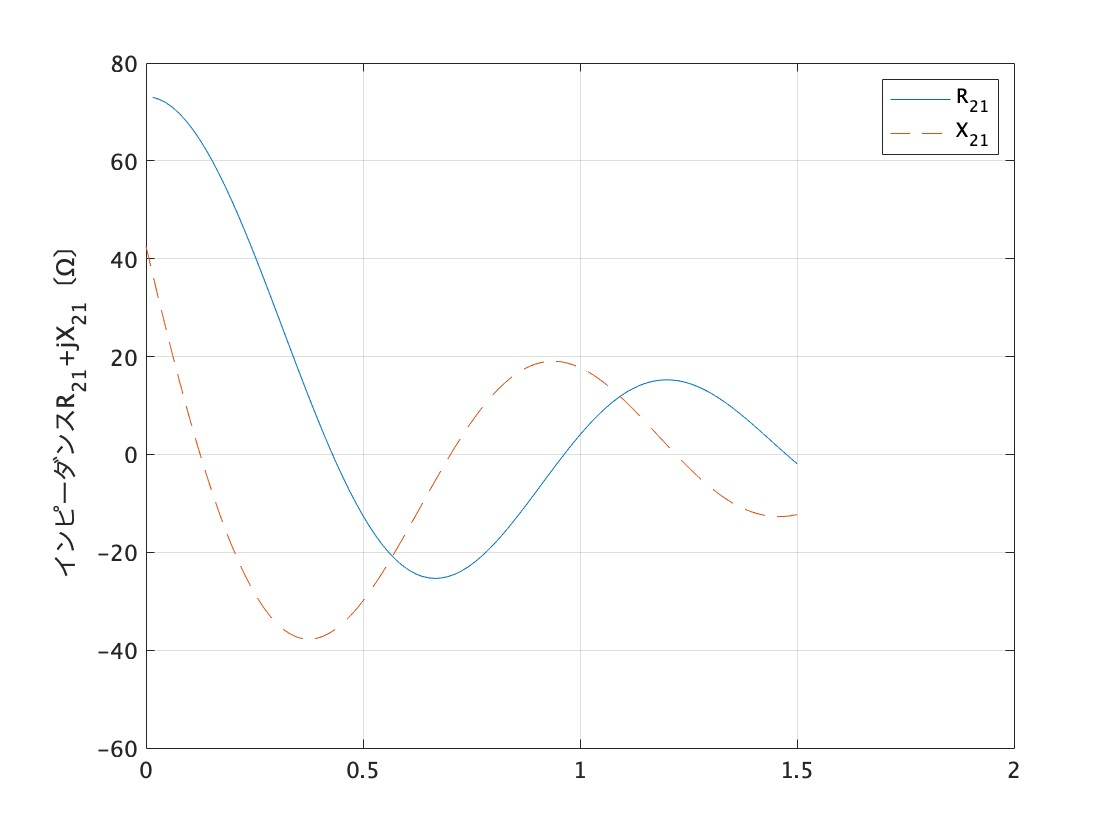
\includegraphics[keepaspectratio,scale=0.2]{pic1.jpg}
      \end{center}
      \caption{P39 グラフ}
    \end{minipage}
    \begin{minipage}[b]{0.45\linewidth}
    \begin{center}
      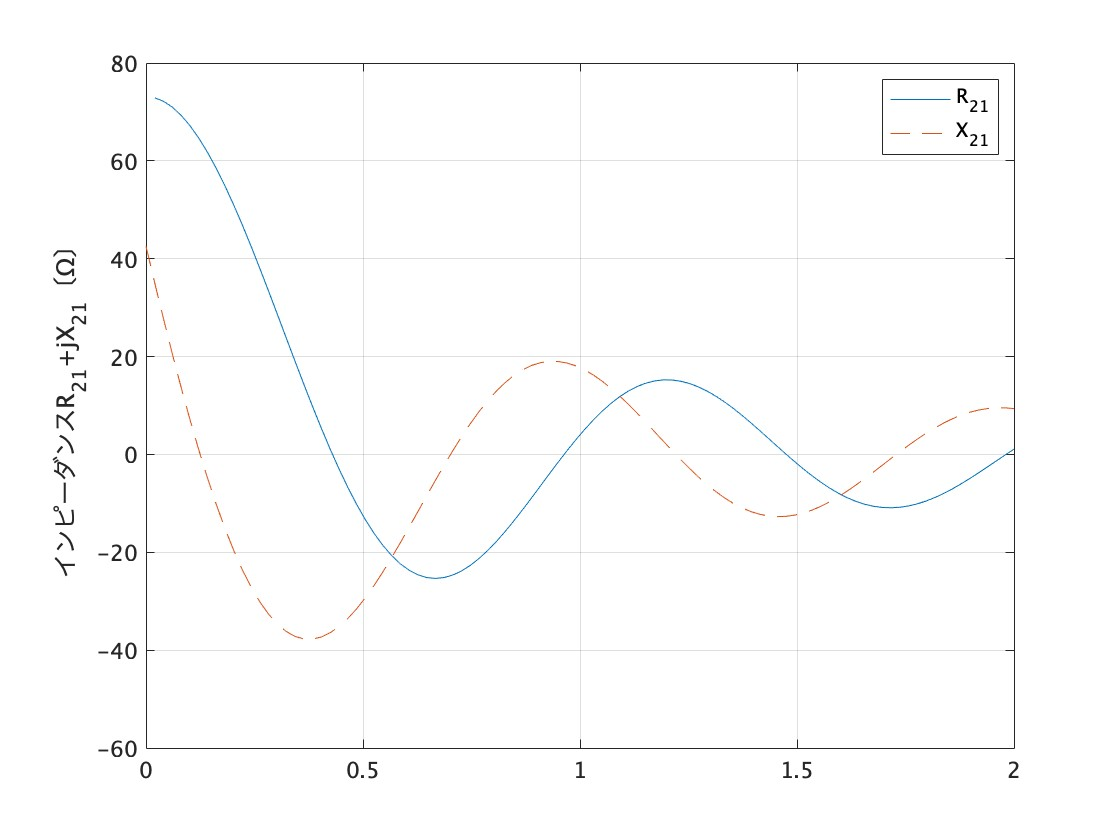
\includegraphics[keepaspectratio,scale=0.2]{pic2.jpg}
      \end{center}
      \caption{演習問題4}
    \end{minipage}
  \end{figure}



\end{document}

